\originalchapter{2019 年作业一}
\label{ass:ps1}
题源: MIT 18.335J Spring 2019, PS1. 本章解答按 Steven G. Johnson 的答案 PDF 与官方 PS1 答案 notebook 译审; 原作业要求 Julia, 本册用 Julia 1.10.10 标准库实际运行随附 \texttt{assessment\_checks.jl}, 另以 Python 高精度计算复核; 未把原 notebook 的运行记录当作本次实跑记录.
\originalsection{浮点表示与函数计算}
\begin{exercise}\label{ps1:q1}
原题只引用 Trefethen/Bau 13.2, 并说明 (c) 可用 Julia, 需区分整数 \texttt{2\^{}50} 和浮点 \texttt{2.0\^{}50}. 原教材完整题面未取得. 以下仅整理 MIT 官方答案明确讨论的最小不可精确表示正整数及其验证, 不补造教材其他子问.
\end{exercise}
\begin{solution}
基数 $\beta$、$t$ 位有效数字且指数范围足够时, $1,\ldots,\beta^t$ 都能精确表示; $\beta^t=\beta^{t-1}\beta$ 可把末位零吸收进指数. 区间 $[\beta^t,\beta^{t+1})$ 的浮点间距为 $\beta$, 因而最小不可表示正整数为 $\beta^t+1$. IEEE binary32 为 $2^{24}+1=16777217$, binary64 为 $2^{53}+1=9007199254740993$. 对整数 $i=2^{53}+o$, $o=-3,\ldots,3$, 比较 $i$ 与浮点结果转回整数的值, 得到依次为真、真、真、真、假、真、假. 不要把 $i$ 先转浮点再比较两个浮点值.
\end{solution}
\begin{exercise}\label{ps1:q2}
(a) 编写 $L_4(x,y)=(|x|^4+|y|^4)^{1/4}$, 检查 $(10^{-100},0)$ 与 $(10^{100},0)$ 的结果. 不用任意精度计算, 修改算法, 使双精度输入的相对误差在几个机器精度的量级; 可用高精度参考检验.
(b) 编写 $\operatorname{cotdiff}(x,y)=\cot x-\cot(x+y)$, 检查 $(1,10^{-20})$. 不用任意精度计算, 改写算法以避免 $|y|\ll|x|$ 时的消去, 同时考虑 $x,y$ 可比的情况. 可用三角恒等式或小量 Taylor 展开.
\end{exercise}
\begin{solution}
(a) 直接四次方分别下溢为零和上溢为无穷. 令 $s=\max(|x|,|y|)$, $s=0$ 时返回零, 否则计算
\[
 L_4=s\bigl[(|x|/s)^4+(|y|/s)^4\bigr]^{1/4}.
\]
括号内至少一项为 1, 总和在 $[1,2]$, 不再出现主导项的中间溢出. 小项下溢时其贡献已低于舍入精度. 两个指定例子分别返回 $10^{-100},10^{100}$. 若真实答案本身超出有限浮点范围, 无法要求有限值的相对精度; 次正规区应以绝对误差或 ulp 衡量, 不能无条件断言相对误差为 $O(u)$.

(b) 直接算法返回零. 利用恒等式
\[
 \cot x-\cot(x+y)=\frac{\sin y}{\sin x\sin(x+y)}.
\]
避免两个几乎相等余切相减; 指定输入给出约 $1.412282927437392\times10^{-20}$. 实现可按 $(\sin y/\sin x)/\sin(x+y)$ 计算, 避免分母乘积无谓下溢. 官方 notebook 另用 $(\cot(x+y)\cot x+1)\tan y$, 对该小量例子准确, 但在 $y$ 接近 $\pi/2$ 时引入不必要的极点; 正弦式不含这一人为极点. 原函数在 $\sin x=0$ 或 $\sin(x+y)=0$ 处无定义. 当 $x+y$ 接近极点、输入加法改变距极点的距离时, 舍入输入会被条件数放大; 任何双精度公式都不能保证所有此类输入几 ulp 的相对误差. 这里给的是消去问题的修复及明确的适用边界.
\end{solution}
\originalsection{二阶 Taylor 求根与成对求和}
\begin{exercise}\label{ps1:q3}
已知解析函数 $f,f',f''$, 普通 Newton 法为 $x_{n+1}=x_n-f(x_n)/f'(x_n)$.
(a) 用二阶 Taylor 近似设计利用三个函数值的迭代, 求二次方程根时应避免消去, 必要时回退普通 Newton 步.
(b) 对根 $\alpha$ 分析 $x_n=\alpha(1+\delta_n)$ 的渐近收敛率.
(c) 修改课堂求根程序, 对 $f(x)=x^3-1$, 从 $x_1=2$ 出发用高精度计算误差 $x_n-1$, 验证预测的阶数; 准确十进制位数约为 $-\log_{10}|x_n-1|$.
\end{exercise}
\begin{solution}
(a) 在当前点令 $a=f(x)$、$b=f'(x)$、$c=f''(x)$, 解 $a-bd+cd^2/2=0$. 取趋近于 Newton 步 $a/b$ 的小根, 用有理化形式
\[
 d=\frac{2a}{b+\operatorname{sign}(b)\sqrt{b^2-2ac}},\qquad x_{\rm new}=x-d.
\]
实数判别式为负则回退 $d=a/b$; $a=0$ 时停止, $b=0$ 时需另选起点或保护策略. 此局部方法假设简单根 $f'(\alpha)\ne0$.

(b) 令 $e=x-\alpha$. 小根满足 $d=e+O(e^2)$; 对 $f(x-d)$ 在 $x$ 展开, 二阶项之和按构造为零, 故
\[
 f(x-d)=-\frac{f'''(x)}6d^3+O(d^4),\qquad
 e_{\rm new}=-\frac{f'''(\alpha)}{6f'(\alpha)}e^3+O(e^4).
\]
因而一般为三阶收敛; 首项系数为零时还可能更高. 若 $\alpha\ne0$, 则 $\delta_{n+1}=-\alpha^2 f'''(\alpha)\delta_n^3/(6f'(\alpha))+O(\delta_n^4)$. 根为零时应使用绝对误差 $e$, 不使用相对记号.

(c) 此例首项系数为 $-1/3$. 初始点的判别式 $144-168<0$, 第一轮回退给 $x=17/12$. 后续准确位数约为 $0.3802,1.5114,5.0108,15.5097,47.0061,141.4954$, 渐近每轮增至约三倍. 随附 Julia 脚本用 BigFloat 高精度实跑, Python 脚本用 Decimal 复核并输出 $e_{n+1}/e_n^3\to-1/3$; 高精度只用于本问验证, 不作为 (a) 的避免消去手段.
\end{solution}
\begin{exercise}\label{ps1:q4}
计算 $\sum_{i=1}^n x_i$, 递归二分输入并将两半的和相加; 空输入返回零, 单元素返回该元素.
(a) 当 $n$ 为 2 的幂时证明误差不超过 $u\log_2n\sum_i|x_i|+O(u^2)$, 而非朴素求和的线性增长.
(b) 有人担心每个元素一次函数调用会很慢. 修改实现, 在保留对数误差界的同时使性能接近循环求和.
(c) 修改官方 notebook 的单精度 \texttt{div2sum}, 在更大长度范围对随机输入画误差曲线, 判断与理论是否相符.
\end{exercise}
\begin{solution}
(a) 假设无溢出且标准相对误差模型适用. 每个叶子经历 $h=\log_2 n$ 次舍入, 故 $\widetilde s=\sum_i x_i\prod_{j=1}^{h}(1+\eta_{ij})$, $|\eta_{ij}|\le u$. 由乘积误差引理, $|\widetilde s-s|\le\gamma_h\sum_i|x_i|$, $\gamma_h=hu/(1-hu)$, 给出所需一阶界; $O(u^2)$ 中的常数依赖固定 $n$.

(b) 用固定阈值 $N$ (如 200): 长度小于 $N$ 时循环求和, 否则二分. 每个叶子经历至多 $N-1+\lceil\log_2(n/N)\rceil$ 次舍入 (小 $n$ 时用 $N-1$ 的界), 仍为 $O(\log n)$; 调用数降到 $O(n/N)$. 这改善调用开销, 实际时钟速度依赖编译器、向量化与实现.

(c) 脚本固定随机种子, 用 binary32 的每次加法分别执行逐项、纯成对、阈值成对三种算法, 以对同一 binary32 输入的 Float64 求和作参考, 长度覆盖 $2^4$ 到 $2^{18}$. 图中误差均低于相应 $\gamma_h\sum|x_i|$ 界, 阈值法保留对数阶的界. 单组随机数据的误差无需单调增长, 也不能凭曲线证明最坏界. 图中数据来自本次 Julia 实跑; 没有据此宣称性能倍数.
\begin{center}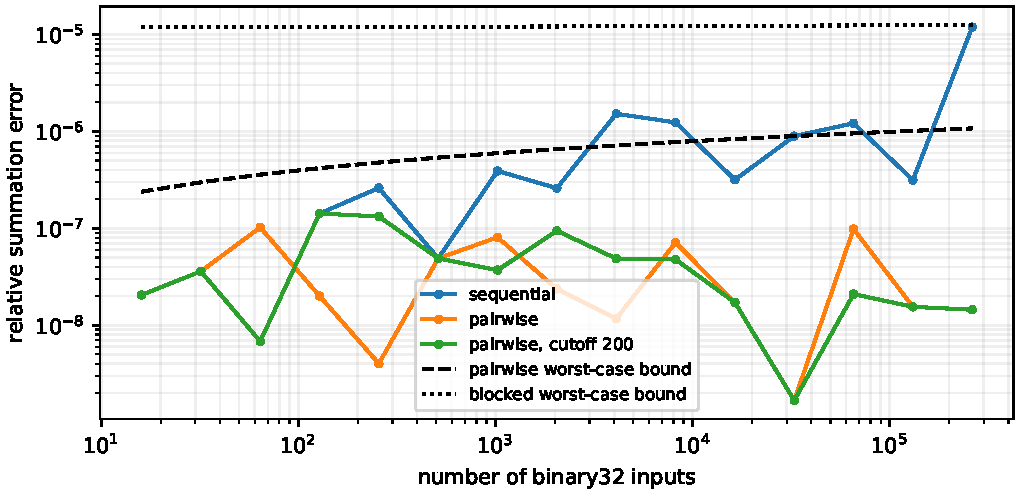
\includegraphics[width=.78\linewidth]{experiments/assessment-summation.pdf}\end{center}
\end{solution}
